%\section{Derivatives of Functions}
\vspace{-0.25 in}
\begin{framed}
\subsection*{Objectives}
\begin{itemize}
    \item Understand the difference between average velocity and instantaneous velocity.
    \item Understand the method for determining the \textbf{slope} of the graph of a function at a specific point using limits.
    \item Understand how the \textbf{derivative} of a function can be used to determine the slope of the graph of a function at any point.
\end{itemize}

%%%Reading Assignment%%%
\subsection*{Suggested Reading:}
\begin{itemize}
\item \cite{Calaway}
    \begin{itemize}
        \item \emph{Precalculus Idea: Slope and Rate of Change} in Lesson 1 of Chapter 1 (page 73)
        \item Lesson 2 of Chapter 1 (pages 80-92)
        
    \end{itemize}
\item \cite{Hoffman}
    \begin{itemize}
        \item \emph{Which functions have derivatives? differentiability implies continuity} in section 3.3 (pages 272-274)
    \end{itemize}
\end{itemize}
%\subsection*{Supplemental Materials:}
%%%Key Terms%%%
\subsection*{Key Terms:} 

\begin{multicols}{2}
\begin{itemize}
    \item slope of a secant line
    \item slope of a tangent line
    \item derivative of a function; differentiation
    \item slope of a curve using the derivative.
\end{itemize}
\end{multicols}
\end{framed}

\newpage
%\noindent\makebox[\linewidth]{\rule{\textwidth}{0.8pt}}
\noindent The \textbf{derivative of a function} is a topic that we will not stop discussing in this class.  It will allow us to analyze the behavior of functions in a much more detailed manner than we were able to do using only the concepts developed in College Algebra.  The importance of derivatives cannot be overstated.  We will need to start out using an intuitive approach to determine a derivative, but we will see in subsequent sections that finding derivatives will be much easier and more efficient as we learn more sophisticated techniques of differentiation.  \\

\noindent \underline{Slope and Rate of Change:}The slope of a line measures how fast a \emph{line} rises or falls as we move from left to right along the line.  It measures the rate of change of the y-coordinate with respect to changes in the x-coordinate. If the line represents the distance traveled over time, for example, then its slope represents the \textbf{velocity}.\\

\noindent \underline{The geometric interpretation:} The goal is determine the \textbf{slope of a curve} at a point.  We have defined this slope to be the slope of the \textbf{tangent line} to the curve at the point of interest. \\

\begin{wrapfigure}[4]{r}{0.45\textwidth}

\begin{figure}[H]
\center
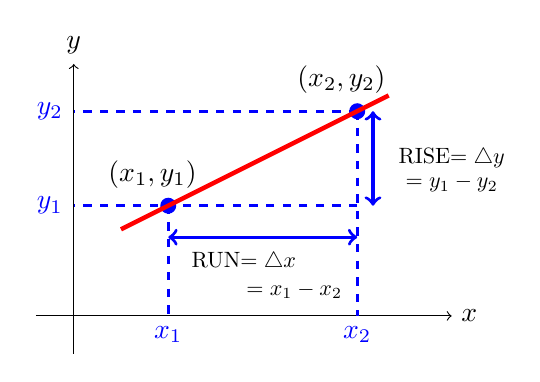
\begin{tikzpicture}[scale =0.8]
\draw[->] (-0.6,0) -- (6,0) node[right,scale=1]{$x$};
\draw[->] (0,-0.6) -- (0,4) node[above,scale=1]{$y$};

\draw[blue, very thick, dashed] (1.5,7/4)--(1.5,0)  node[below,scale=1]{$x_1$};
\draw[blue, very thick, dashed] (4.5,3.25)--(4.5,0)  node[below,scale=1]{$x_2$};
\draw[blue, very thick, dashed] (4.5,7/4)--(0,7/4)  node[left,scale=1]{$y_1$};
\draw[blue, very thick, dashed] (4.5,3.25)--(0,3.25)  node[left,scale=1]{$y_2$};

\draw[blue, very thick, fill]  (4.5,3.25) circle[radius=.1];
\node[scale=1] at (4.25,3.75) {$(x_2,y_2)$};
\draw[blue, very thick, fill]  (1.5,7/4) circle[radius=.1];
\node[scale=1] at (1.25,2.25) {$(x_1,y_1)$};

\draw[<->][blue, very thick] (1.5,1.25) -- (4.5,1.25);
\node[scale=0.8] at (2.7,0.85) {RUN$=\triangle x$};
\node[scale=0.8] at (3.5,0.4) {$=x_1-x_2$};

\draw[<->][blue, very thick] (4.75,3.25) -- (4.75,1.75);
\node[scale=0.8] at (6,2.5) {RISE$=\triangle y$};
\node[scale=0.8] at (6,2.1) {$=y_1-y_2$};


\draw[domain=.75:5, smooth, variable=\x, red, ultra thick] plot ({\x}, {(0.5*\x+1});


\end{tikzpicture}
\caption{Calculate slope using two points on the line}
\label{fig:line}
\end{figure}
\end{wrapfigure}

\noindent Figure \ref{fig:line} reminds you how to calculate slope ($m$) using two points on the line:
\begin{equation}
    m=\frac{rise}{run}=\frac{\triangle y}{\triangle x}=\frac{y_2-y_1}{x_2-x_1}=\frac{y_1-y_2}{x_1-x_2}
\end{equation}
\hfill \break
\hfill \break
\hfill \break
\hfill \break
\hfill \break
\hfill \break



\begin{multicols}{2}

\begin{minipage}{0.35\textwidth}

\begin{figure}[H]
    
    \begin{tikzpicture}[scale =0.5]
    \draw[->] (-1.5,0)--(4,0) node[right]{$x$};
    
     \draw[thick] (1,0.1)-- (1,-0.1) node[below]{1};
     \draw[thick] (2,0.1)-- (2,-0.1) node[below]{2};
     \draw[thick] (3,0.1)-- (3,-0.1) node[below]{3};
    
     
    \draw[->] (0,-0.5)--(0,10) node[above]{$x$};
    \draw[thick] (0.1,9)-- (-0.1,9) node[left]{9};
    \draw[thick] (0.1,4)-- (-0.1,4) node[left]{4};
     \draw[thick] (0.1,1)-- (-0.1,1) node[left]{1};
    \draw[domain=-1:3.15, smooth, variable=\x, red, thick] plot ({\x}, {(\x)^2});
    \draw[black, very thick, fill]  (2,4) circle[radius=.1];
    \draw[domain=1.2:3, dashed, variable=\x, black, ultra thick] plot ({\x}, {(4*\x)-4});
    \draw[blue, very thick, fill]  (3,9) circle[radius=.1];
    \draw[domain=1.7:3.3, dashed, variable=\x, blue, ultra thick] plot ({\x}, {(6*\x)-9});
    \node[scale=1] at (2.7,1) {$y=x^2$}
    \end{tikzpicture}
    \caption{Calculate slope on a curve}
    \label{fig:curve1}
\end{figure}
\end{minipage}

\begin{minipage}{0.55\textwidth}
\vspace{0.7cm}
\noindent But if we wants to know how fast a \emph{curve} rises or falls, what should we do? The answer is to find the slope of the curve as in Figure \ref{fig:curve1} . There are two ways to find the slope of the curve: 

\begin{enumerate}[leftmargin=*]
    \item Determine the \textbf{slope of a secant line} \emph{passing through} two points on the curve. The slope tells us the \textbf{average velocity} between the points (i.e. how fast the curve rise (or fall) between the points).
    \item Determine the \textbf{slope of a tangent line} which \emph{touches} one point on the curve. The slope tells us the instantaneous velocity (i.e. how fast the curve rise (or fall) \textbf{at} the points).
\end{enumerate}
\end{minipage}
\end{multicols}
%\hfill \break

\begin{tcolorbox}[title = {Average Velocity (Rate of Change) vs.  Instantaneous Velocity (Rate of Change)}]
\textbf{Average Velocity} = $\frac{\triangle position}{\triangle time}$ = Slope of the \textbf{secant line} through 2 points.\\\\
\textbf{Instantaneous Velocity} = Slope of the \textbf{tangent line} to the graph.
\end{tcolorbox}

\noindent \underline{Approximate the slope of a Tangent Line from the slope of a secant line} by using the idea that secant lines over tiny intervals approximate the tangent line. 

\Opensolutionfile{ans}[ans2]
\Opensolutionfile{ansL}[ansL2]
\begin{example}\label{approxTangent1}
Approximate the slope of the tangent line at $(2,4)$ from the slope of the secant line passing through $(2,4)$ and $(3,9)$.\\
%%short answer
    \begin{sol}
    5
    \end{sol}
    %%solution
    \begin{solL}
    Let \(f(x)=\sqrt{25-x^2}\). So, $\lim\limits_{x \to -1} f(x)=f(4)=\sqrt{25-4^2}=3$. test
    
    \end{solL}
\end{example}
\vspace{1in}

\begin{example}\label{approxTangent2}
Approximate the slope of the tangent line at $(2,4)$ from the slope of the secant line passing through $(2,4)$ and $(2.5,6.25)$.\\
%%short answer
    \begin{sol}
    4.5
    \end{sol}
    %%solution
    \begin{solL}
    Let \(f(x)=\sqrt{25-x^2}\). So, $\lim\limits_{x \to -1} f(x)=f(4)=\sqrt{25-4^2}=3$. test
    
    \end{solL}
\end{example}
\vspace{1in}

\begin{example}\label{approxTangent3}
Compare the two secant lines in Example \ref{approxTangent1} and in Example \ref{approxTangent2}.  Which would be a better approximation of the tangent line to the curve at 
$(2,4)$? Why?\\
%%short answer
    \begin{sol}
    The secant line in Example \ref{approxTangent2}.
    \end{sol}
    %%solution
    \begin{solL}
    The secant line passing through $(2,4)$ is a better approximation because of its smaller interval. As the interval got smaller and smaller, the secant line got closer to the tangent line and its slope got closer to the slope of the tangent line.  
    
    \end{solL}
\end{example}
\vspace{0.8in}

\noindent As the interval got smaller and smaller, the secant line got closer to the tangent line and its slope got closer to the slope of the tangent line.  We can continue picking points closer and closer to $(2,4)$ on the graph of  the function $f$, and then calculating the slopes of the lines through each of these points and the point $(2,4)$. 
%%%%%%%%%%%%%%%%%%%%%%%%%%%%%%%%%%%%%%%%%%%%%%%%%%%%%%%%%%%%%%%%%%%%%%%%
\vspace{-0.25cm}
\begin{table}[H]
\begin{center}
\begin{tabular}{ |p{2cm}|p{2cm}|p{2cm}|p{2cm}|p{2cm}|p{2cm}| }
 \hline
 \multicolumn{3}{|c|}{Point to the left of (2,4)}& \multicolumn{3}{c|}{Point to the right of (2,4)} \\

\hline

$x$ & $y=x^2$& Slope &$x$ & $y=x^2$& Slope   \\
\hline
1.5 & 2.25 & 3.5 & 3 & 9 & 5  \\
\hline
1.9 & 3.61 & 3.9 & 2.5 & 6.25 & 4.5  \\
\hline
1.99 & 3.9601 & 3.99 & 2.01 & 4.0401 & 4.01  \\

\hline
\end{tabular}
\caption{}
\label{table:exTangSlope}
\end{center}

\end{table}

\vspace{-0.75cm}
\begin{example}\label{approxTangent4}
Using Table \ref{table:exTangSlope} above, guess the value of the slope of the tangent line at $x=2$.\\
%%short answer
    \begin{sol}
    2
    \end{sol}
    %%solution
    \begin{solL}
     
    
    \end{solL}
\end{example}
\newpage

\begin{wrapfigure}[12]{l}{0.65\textwidth}

\begin{figure}[H]
\center
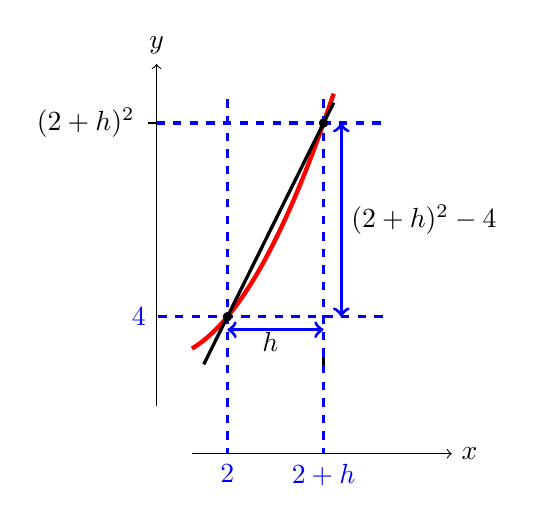
\begin{tikzpicture}[scale =1.5]
\draw[->] (0.3,-0.8) -- (2.5,-0.8) node[right,scale=1]{$x$};
\draw[->] (0,-0.4) -- (0,2.5) node[above,scale=1]{$y$};

\draw[thick] (0.075,2)-- (-0.075,2) node[scale=1] at (-0.6,2) {$(2+h)^2$};

\draw[domain=0.3:1.5, smooth, variable=\x, red, ultra thick] plot ({\x}, {(\x)^2});

\draw[thick] ({sqrt(2)},0.075)-- ({sqrt(2)},-0.075);
\draw[blue, very thick, dashed] ({sqrt(2)},2.2)--({sqrt(2)},-0.8)  node[below,scale=1]{$2+h$};
\draw[blue, very thick, dashed] (0.6,2.2)--(0.6,-0.8)  node[below,scale=1]{2};
\draw[blue, very thick, dashed] ({sqrt(2)+0.5},0.36)--(0,0.36) node[left,scale=1]{4};
\draw[blue, very thick, dashed] (0,2)--({sqrt(2)+0.5},2);

\draw[domain=0.4:1.5, variable=\x, black, very thick] plot ({\x}, {(2.014214*\x)-0.84853});

\draw[very thick, fill]  (0.6,0.36) circle[radius=.025];
\draw[very thick, fill]  ({sqrt(2)},2) circle[radius=.025];


\draw[<->][blue, very thick] (0.6,0.25) -- ({sqrt(2)},0.25);
\node[scale=1] at ({sqrt(2)-0.45},0.15) {$h$};

\draw[<->][blue, very thick] ({sqrt(2)+0.15},0.36) -- ({sqrt(2)+0.15},2);
\node[scale=1] at ({sqrt(2)+0.85},{(0.36+2)/2}) {$(2+h)^2-4$};

\end{tikzpicture}
\caption{\footnotemark }
\label{fig:secantLimit}
\end{figure}
\end{wrapfigure}

\noindent We can bypass much of the calculating by not picking the points one at a time:  let's look at a general point near $(2,4)$.  Define  $x = 2 + h$  so $h$ is the increment from 2 to  $x$  (Figure \ref{fig:secantLimit}).  If $h$ is small, then $x = 2 + h$ is close to  2 and the point  $(2+h, f(2+h)) = (2+h, (2+h)^2 )$  is close to $(2,4)$.  
\footnotetext{From \cite{Calaway} ;  page 85}
\hfill \break
\hfill \break
\hfill \break
\hfill \break
\hfill \break
\hfill \break




\noindent \underline{Secant lines and limits:}  We now indicate, mathematically, how we will determine the slope of the tangent line to the curve at an arbitrary point.  The end result will be a \textbf{function} that we will refer to as \emph{“the derivative of} $f(x)$”, denoted by $f^\prime (x)$ (\emph{read aloud as "}$f$ \emph{prime of} $x$).  The derivative function will take a value of $x$ as an input and provide the slope of the graph of $f(x)$ at that point as the output. \\

\begin{tcolorbox}[title = {Notation of Derivatives}]
The derivative of \(y = f(x)\) with respect to \(x\) is written as\\
$f^\prime (x)$ (read aloud as "$f$ \emph{prime of} $x$") or \(\displaystyle\frac{dy}{dx}\) (read aloud as \emph{"dee why dee ex"}). \\
In verb forms, we say we \textbf{find the derivative} of a function, or \textbf{take the derivative} of a function, or \textbf{differentiate} a function.
\end{tcolorbox}

\vspace{0.25cm}

\begin{tcolorbox}[title = {Formal Algebraic Definition of Derivatives}]
\begin{equation}\label{eq:dervLimit}
f'(x)=\lim\limits_{h \to 0} \displaystyle\frac{f(x+h)-f(x)}{h}
\end{equation} 
\end{tcolorbox}

\vspace{0.25cm}

\begin{tcolorbox}[title = {Practical Definition of Derivatives}]
The derivative can be approximated by looking at an average rate of change, or the slope of a secant line, 
over a very tiny interval.  The tinier the interval, the closer this is to the true instantaneous rate of change, slope of the tangent line, or slope of the curve.

\end{tcolorbox}
\newpage
%%%Examples%%%

%exexexexexexexexexexexexexexexexexexexex
\begin{example}
%%%%%%%%%%%%%%Alternative Option%%%%%%%%%%%%%
\begin{comment}
Use the the \textbf{limit} definition of the derivative  in the equation \ref{eq:dervLimit} (page \pageref{eq:dervLimit}) to \textbf{determine the derivative}, $f^\prime(x)$, for the function \(f(x)=x^2+3\).
\begin{center}
$f^\prime(x)=\rule{5cm}{0.25mm}$
\end{center}
Then, answer the following questions: 
\end{comment}
%%%%%%%%%%%%%%%%%%%%%%%%%%%%%%%%%%%%
Given the function \(f(x)=x^2+3\), answer the following questions:
\begin{enumerate}
    \item Using the \textbf{limit} definition of the derivative in the equation \ref{eq:dervLimit} (page \pageref{eq:dervLimit}), determine the equation of the derivative, $f^\prime(x)=\rule{5cm}{0.25mm}$.
    \item Find the slope of the graph of $f(x)$ at $x=3$, $x=-1$, and $x=0$. 
    \item How does the \textbf{sign of the derivative} relate to the \textbf{sign of the tangent line}?
    \item What is the sign of the slope of a tangent line at any point on $(-\infty,0)$ ? Is the function \(f\) increasing or decreasing on this interval?
     \item What is the sign of the slope of a tangent line at any point on $(0,\infty)$ ? Is the function \(f\) increasing or decreasing on this interval?
\end{enumerate}
 \vspace{-0.5cm}
 
\begin{figure}[h]
\hspace*{-9cm}
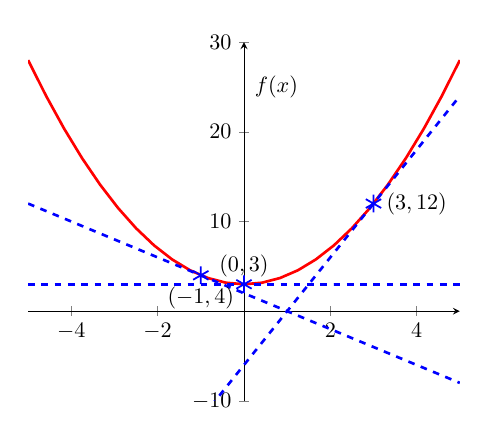
\begin{tikzpicture}[scale=0.8]
\begin{axis}[
    axis lines = middle,
    ymin=-10,ymax=30,
    %xlabel = $x$,
    %ylabel = {$f(x)$},
]

\addplot[color=red, very thick,]{x^2+3};
\addplot[color=blue,dashed, very thick,]{-2*x+2}; 
\addplot[color=blue,dashed, very thick,]{6*x-6};  
\addplot[color=blue,dashed, very thick]{3};  
\addplot[
    color=blue,
    only marks,
    mark=asterisk, thick,
    mark size=4pt,
    ]
    coordinates {
    (-1,4)(0,3)(3,12) 
    };
    \node at (axis cs:4,12) {$(3,12)$};
    \node at (axis cs:-1,1.5) {$(-1,4)$};
    \node at (axis cs:0,5) {$(0,3)$};
    \node at (axis cs:0.75,25) {$f(x)$};
    \node at (axis cs:5.5,0) {$x$};

\end{axis}

\end{tikzpicture}
%\hspace*{-6cm}
\captionsetup{justification=justified, singlelinecheck=false}
\caption{Graph of $f(x)$ with tangent lines at $x=-1$,\\ $x=0$ and $x=3$}
\label{fig:derivativeLimit}

\end{figure}
%\vspace{1cm}
    %%short answer
    \begin{sol}
    $f'(x)=2x$; (1) 6, -2, 0; (2) same sign; (3) negative;decreasing (4) positive;increasing. 
    \end{sol}
    %%solution
    \begin{solL}
    \hfill
        \begin{figure}[h!]
        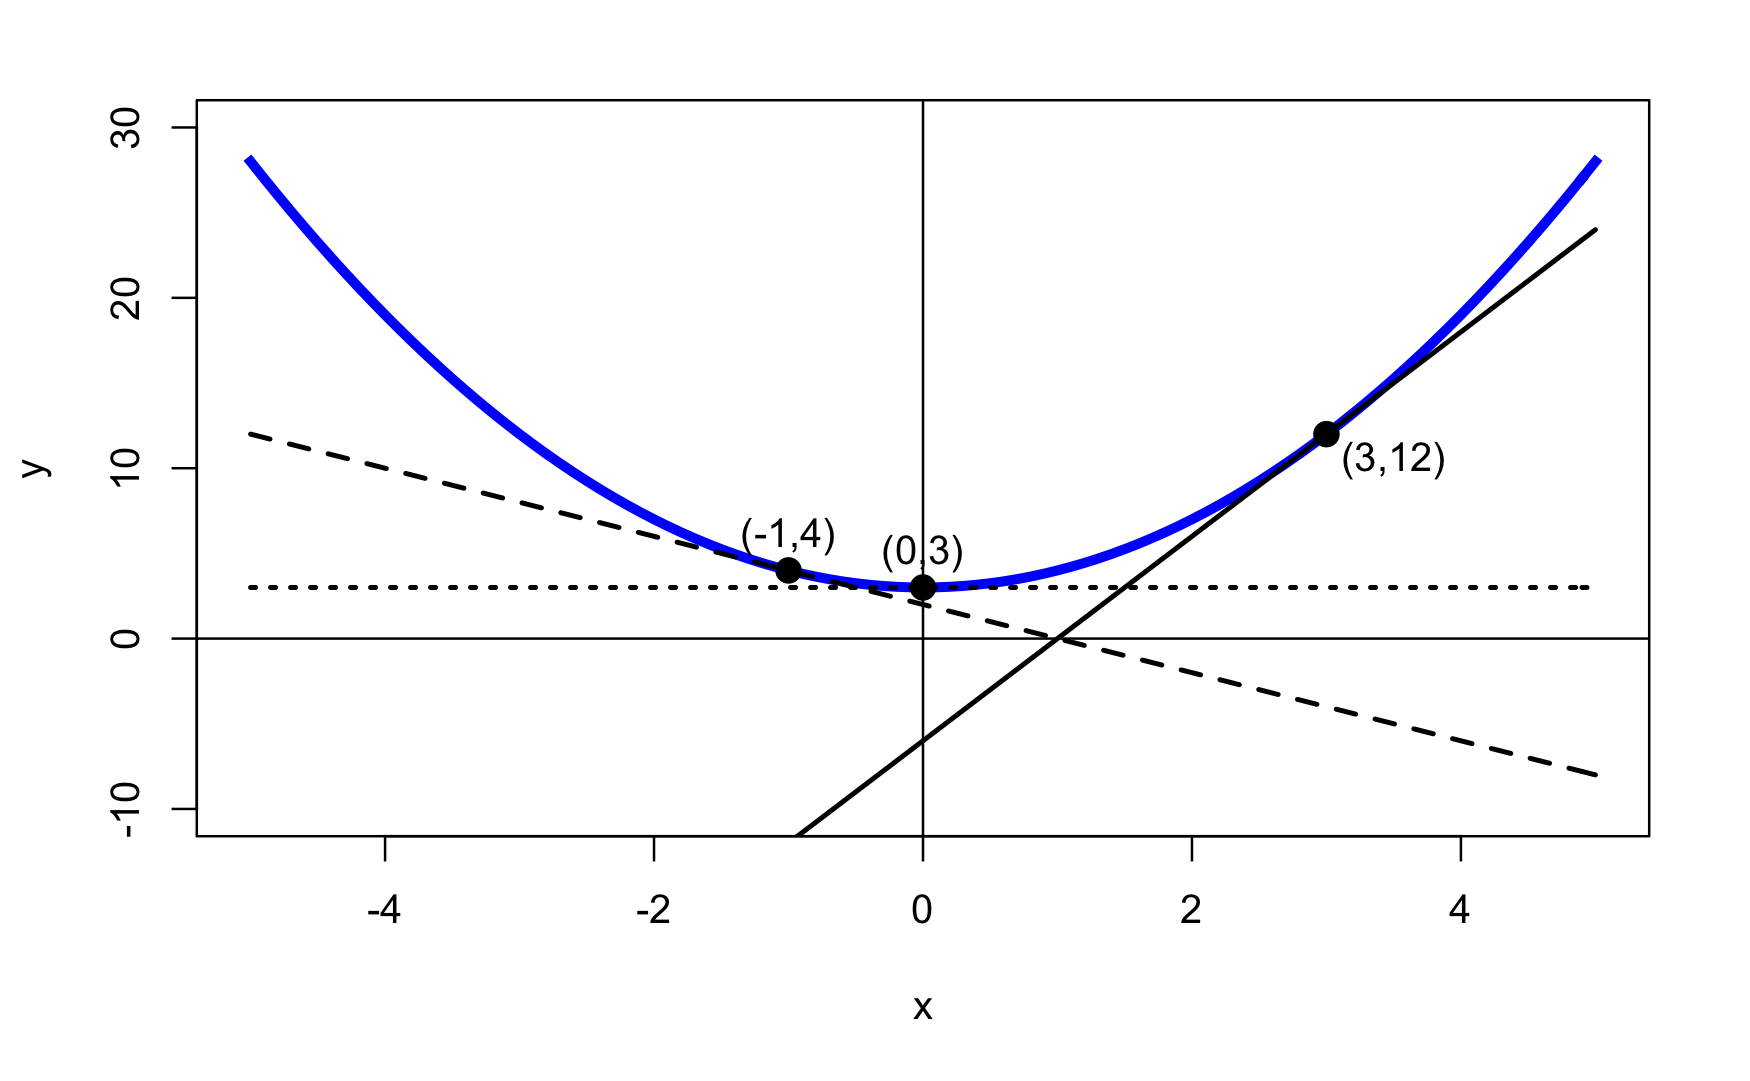
\includegraphics[width=0.8\textwidth]{derivatives-functions/derivativeLimit}
        \centering
    \end{figure}
    
    \end{solL}
    
\end{example}

%exexexexexexexexexexexexexexexexexexexex
%Hoffman (3.3 Shape of a Graph; Second Shape Theorem  pg.275 )
%Calaway (The Derivative as a Function (pg.87-88))
\begin{tcolorbox}[title = {The Derivative and The Behavior of a Function}]
For a function \(f\) which is \emph{differentiable}\footnotemark on an interval \(I\):
\renewcommand{\labelenumii}{\roman{enumii}}
\begin{enumerate}
    \item if \(f'(x)>0\) for all \(x\) in the interval \(I\), then \(f\) is increasing on \(I\).
     \item if \(f'(x)<0\) for all \(x\) in the interval \(I\), then \(f\) is decreasing on \(I\).
      \item if \(f'(x)=0\) for all \(x\) in the interval \(I\), then \(f\) is constant on \(I\).
\end{enumerate}

\end{tcolorbox}

\noindent The derivative of a function tells about the general shape of the function, and we can use that shape information to determine if an extreme point is a maximum or minimum or neither (See Figure \ref{fig:dervBeh}\footnotemark).

\begin{figure}[H]
\center
\begin{minipage}{0.235\textwidth}
\begin{center}
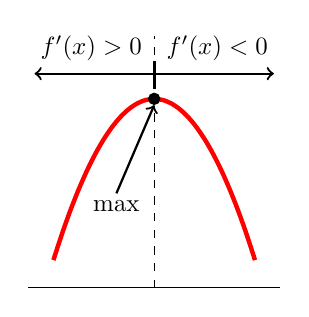
\begin{tikzpicture}[scale =0.8]
\draw[-] (-2,0) -- (2,0);
\draw[dashed] (0,0) -- (0,4);
\draw[domain=-1.6:1.6, smooth, variable=\x, red, ultra thick] plot ({\x}, {(-(\x)^2+3});
\draw[very thick, fill]  (0,3) circle[radius=.07];
\draw[->,thick] (-0.6,1.5) -- (0,2.9);
\node[scale=0.9] at (-0.6,1.3) {max};
\draw[<-,thick] (-1.9,3.4) -- (0,3.4) ;
\node[scale=0.9] at (-1,3.8) {$f'(x)>0$};
\draw[-,very thick] (0,3.6) -- (0,3.15) ;
\draw[->,thick] (0,3.4) -- (1.9,3.4) ;
\node[scale=0.9] at (1,3.8) {$f'(x)<0$};


\end{tikzpicture}
\end{center}
\end{minipage}
\hspace{0.05cm}
\begin{minipage}{0.235\textwidth}
\begin{center}
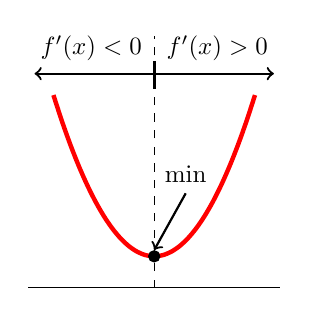
\begin{tikzpicture}[scale =0.8]
\draw[-] (-2,0) -- (2,0) ;
\draw[dashed] (0,0) -- (0,4) ;
\draw[domain=-1.6:1.6, smooth, variable=\x, red, ultra thick] plot ({\x}, {((\x)^2+0.5});
\draw[very thick, fill]  (0,0.5) circle[radius=.07];
\draw[->,thick] (0.5,1.5) -- (0,0.6);
\node[scale=0.9] at (0.5,1.8) {min};
\draw[<-,thick] (-1.9,3.4) -- (0,3.4) ;
\node[scale=0.9] at (-1,3.8) {$f'(x)<0$};
\draw[-,very thick] (0,3.6) -- (0,3.15) ;
\draw[->,thick] (0,3.4) -- (1.9,3.4) ;
\node[scale=0.9] at (1,3.8) {$f'(x)>0$};
\end{tikzpicture}
\end{center}
\end{minipage}
\hspace{0.05cm}
\begin{minipage}{0.235\textwidth}

\begin{center}

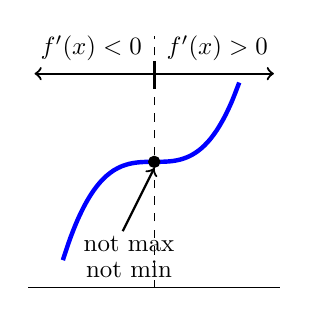
\begin{tikzpicture}[scale =0.8]
\draw[-] (-2,0) -- (2,0) ;
\draw[dashed] (0,0) -- (0,4) ;
\draw[domain=-1.45:1.35, smooth, variable=\x, blue, ultra thick] plot ({\x}, {((0.8*\x)^3+2});

\draw[very thick, fill]  (0,2) circle[radius=.07];
\draw[->,thick] (-0.5,0.9) -- (0,1.9);
\node[scale=0.9] at (-0.4,0.7) {not max};
\node[scale=0.9] at (-0.4,0.3) {not min};
\draw[<-,thick] (-1.9,3.4) -- (0,3.4) ;
\node[scale=0.9] at (-1,3.8) {$f'(x)<0$};
\draw[-,very thick] (0,3.6) -- (0,3.15) ;
\draw[->,thick] (0,3.4) -- (1.9,3.4) ;
\node[scale=0.9] at (1,3.8) {$f'(x)>0$};

\end{tikzpicture}
\end{center}
\end{minipage}
%\hspace{0.05cm}
\begin{minipage}{0.235\textwidth}

\begin{center}

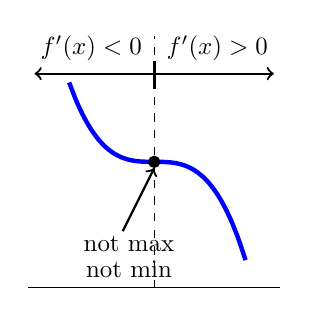
\begin{tikzpicture}[scale =0.8]
\draw[-] (-2,0) -- (2,0) ;
\draw[dashed] (0,0) -- (0,4) ;
\draw[domain=-1.35:1.45, smooth, variable=\x, blue, ultra thick] plot ({\x}, {((-0.8*\x)^3+2});

\draw[very thick, fill]  (0,2) circle[radius=.07];
\draw[->,thick] (-0.5,0.9) -- (0,1.9);
\node[scale=0.9] at (-0.4,0.7) {not max};
\node[scale=0.9] at (-0.4,0.3) {not min};
\draw[<-,thick] (-1.9,3.4) -- (0,3.4) ;
\node[scale=0.9] at (-1,3.8) {$f'(x)<0$};
\draw[-,very thick] (0,3.6) -- (0,3.15) ;
\draw[->,thick] (0,3.4) -- (1.9,3.4) ;
\node[scale=0.9] at (1,3.8) {$f'(x)>0$};

\end{tikzpicture}
\end{center}
\end{minipage}

\caption{} 
\label{fig:dervBeh}

\end{figure}

\footnotetext{See Lesson \ref{differentiability}: Differentiability and Continuity}
\footnotetext{From \cite{Hoffman} ;  page 88}
\newpage
\subsection*{Interpretations of The Derivative }
\vspace{-0.25cm}
%Hoffman (2.1 The Derivative; Interpretations of The Derivative;  pg.140 )
So far we have emphasized the derivative as the slope of the line tangent to a graph . That interpretation is very visual and useful when examining the graph of a function, and we will continue to use it. Derivatives, however,are used in a wide variety of fields and applications, and some of these fields use other interpretations. The
following are a few interpretations of the derivative which are commonly used.\\

\noindent\textbf{\underline{General}}
\begin{justify}
\emph{Rate of Change}: $f'(x)$ is the \textbf{rate of change} of the function at $x$. If the units for $x$ are years and the units for $f(x)$ are people, then the units for $\dfrac{df}{dx}$ are $\dfrac{\text{people}}{\text{year}}$, a rate of change in population.\\
\end{justify}

\noindent\textbf{\underline{Graphical}}
\begin{justify}
\emph{Slope}: $f'(x)$ is the \textbf{slope of the line tangent to the graph of} $\bm{f}$ \textbf{at the point} $\bm{(x,f(x))}.$\\
\end{justify}

\noindent\textbf{\underline{Physical}}
\begin{justify}
\emph{Velocity}: If $f(x)$ is the position of an object at time $x$, then $f'(x)$ is the \textbf{velocity} of the object at time $x$. If the units for $x$ are hours and $f(x)$ is distance measured in miles, then the units for $f'(x)=\dfrac{df}{dx}$ are $\dfrac{\text{miles}}{\text{hour}}$, miles per hour, which is a measure of velocity.\\
\end{justify}

\begin{justify}
\emph{Acceleration}: If $f(x)$ is the velocity of an object at time $x$, then $f'(x)$ is the \textbf{acceleration} of the object at time $x$. If the units for $x$ are hours and $f(x)$ has the units $\dfrac{\text{miles}}{\text{hour}}$, then the units for the acceleration $f'(x)=\dfrac{df}{dx}$ are $\dfrac{\text{miles/hour}}{\text{hour}}=\dfrac{\text{miles}}{\text{hour}^2}$, miles per hour per hour.\\
\end{justify}

\noindent\textbf{\underline{Business}}
\begin{justify}
\emph{Marginal Cost, Marginal Revenue, and Marginal Profit}: In business contexts, the word ``\emph{marginal}" usually means the derivative or rate of change of some quantity. We'll explore these terms in more depth later in the section. Basically, the marginal cost is approximately the \underline{additional} cost of making one more object once we have already made $x$ objects. If the units for $x$ are bicycles and the units for $f(x)$ are dollars, then the units for $\dfrac{df}{dx}$ are $\dfrac{\text{dollars}}{\text{bicycle}}$, the cost per bicycle.
\end{justify}
\newpage
\begin{example}
Suppose the demand curve for widgets was given by \(D(p)=\frac{1}{p}\), where $D$ is the quantity of items widgets, in thousands at a price of $p$ dollars. 
\begin{enumerate}[leftmargin=*]
    \item Evaluate \(f(3)\). Interpret the result in the context.\vspace{\stretch{1.25}}
    \item Determine \(f'(x)\) using the limit definition in the equation \ref{eq:dervLimit} (page \pageref{eq:dervLimit}). \vspace{\stretch{2.5}}
    \item Evaluate \(f'(3)\). Interpret the result in the context.\vspace{\stretch{1}}
    
\end{enumerate}

 %%short answer
    \begin{sol}
    \(f(3)=\frac{1}{3}\);\(f'(x)=\frac{1}{x^2}\);\(f'(3)=\frac{1}{9}\)
    \end{sol}
    %%solution
    \begin{solL}
    See example 3 and example 7 in section 2.2 from \cite{Calaway}.
    \end{solL}
\end{example}

\Closesolutionfile{ans}
\Closesolutionfile{ansL}

%%%Short Answers to Examples%%%
\vspace*{\fill}
\subsection*{Short Answers to Examples}
\vspace{-0.5cm}
\begin{multicols}{2}
\input{ans2}
\end{multicols}


